\documentclass{../khlslides}

\usetikzlibrary{arrows.meta}

\title[ADTs]{ADTs}
\author{Fr\'ed\'eric Vogels}



\newcommand{\drawarray}[2][]{
  \pgfkeys{/tikz/.cd,#1,cell name/.get=\cellname}
  \foreach[count=\i] \val in {#2} {
    \pgfmathparse{int(\i-1)}\let\idx\pgfmathresult
    \pgfmathparse{(\i-1)*1.2}\let\x\pgfmathresult
    \node[anchor=south west,cell] (\cellname\space\i) at (\x,0) {\val};
    \node[index] at (\cellname\space\i.north west) {\tiny\idx};
  }
}

\newcommand{\drawvarray}[2][]{
  \pgfkeys{/tikz/.cd,#1,cell name/.get=\cellname}
  \foreach[count=\i] \val in {#2} {
    \pgfmathparse{int(\i-1)}\let\idx\pgfmathresult
    \pgfmathparse{(\i-1)*-1.2}\let\y\pgfmathresult
    \node[anchor=south west,cell] (\cellname\space\i) at (0,\y) {\val};
    \node[index] at (\cellname\space\i.north west) {\tiny\idx};
  }
}

\pgfkeys{
  /tikz/.cd,
  cell/.style={drop shadow,fill=blue!50,minimum size=.8cm},
  highlighted cell/.style={drop shadow,fill=green!50,minimum size=.8cm},
  index/.style={fill=white,draw},
  box/.style={fill=red!10,drop shadow},
  cell name/.initial=cell
}


\begin{document}

\begin{frame}
  \titlepage
\end{frame}


\begin{frame}
  \frametitle{Probleem: Gelukkige Getallen (VPW2011)}
  \begin{center} \large\bfseries
    De \emph{opvolger} van een getal is de som van zijn cijfers.
  \end{center}
  \vskip4mm
  \[
    \begin{array}{r@{}c@{}lcccccc}
      \mathrm{opvolger}(&11&) & = & 1^2 + 1^2 & = & 1 + 1 & = & 2 \\
      \mathrm{opvolger}(&49&) & = & 4^2 + 9^2 & = & 16 + 81 & = & 97 \\
      \mathrm{opvolger}(&123&) & = & 1^2 + 2^2 + 3^2 & = & 1 + 4 + 9 & = & 14
    \end{array}
  \]
\end{frame}

\begin{frame}
  \frametitle{Probleem: Gelukkige Getallen (VPW2011)}
  \begin{center}
    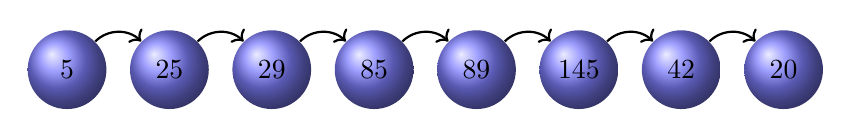
\begin{tikzpicture}[node/.style={ball color=blue!50,circle,minimum size=1cm}]
      \foreach[count=\i] \c in {5,25,29,85,89,145,42,20} {
        \pgfmathparse{\i*1.3}\let\cx\pgfmathresult
        \node[node] (node \i) at (\cx,0) {\c};
      }
      \foreach \i in {1,...,7} {
        \pgfmathparse{int(\i+1)}\let\j\pgfmathresult
        \draw[->,thick] (node \i.north east) to [bend left=45] (node \j.north west);
      }
    \end{tikzpicture}
  \end{center}
  \vskip5mm
  \begin{center}
    \large Ketting van opvolgers
  \end{center}    
\end{frame}

\begin{frame}
  \frametitle{Probleem: Gelukkige Getallen (VPW2011)}
  \begin{center} \Large\bfseries
    \emph{Gelukkig getal}: ketting eindigt op 1.
  \end{center}

  \begin{columns}
    \column{.5\linewidth}
    \begin{center}
      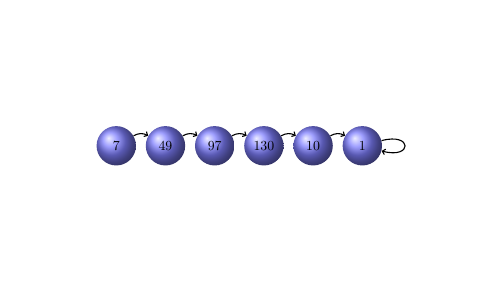
\begin{tikzpicture}[transform shape,scale=0.5,
                          node/.style={ball color=blue!50,circle,minimum size=1cm},
                          arrow/.style={-{Straight Barb[length=1pt]}}]
        \path[use as bounding box] (-1,-3) rectangle (10,3);
        \foreach[count=\i] \c in {7,49,97,130,10,1} { 
          \pgfmathparse{\i*1.25}\let\x\pgfmathresult
          \node[node] (node \i) at (\x,0) {\c};
        }

        \foreach \i in {1,...,5} {
          \pgfmathparse{int(\i+1)}\let\j\pgfmathresult
          \draw[arrow] (node \i) to [bend left=30] (node \j);
        }
        \draw[arrow] (node 6) to [loop right] (node 6);
      \end{tikzpicture}
    \end{center}
    \begin{center} 7 is gelukkig \end{center}

    \column{.5\linewidth}
    \begin{center}
      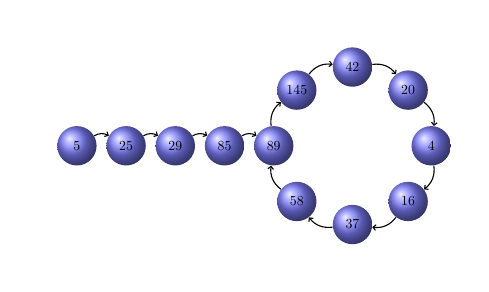
\begin{tikzpicture}[transform shape,scale=0.5,
                          node/.style={ball color=blue!50,circle,minimum size=1cm},
                          arrow/.style={-{Straight Barb[length=1pt]}}]
        \path[use as bounding box] (0,-3) rectangle (11,3);

        \foreach[count=\i] \c in {5,25,29,85} { 
          \pgfmathparse{\i*1.25}\let\x\pgfmathresult
          \node[node] (node \i) at (\x,0) {\c};
        }
        \foreach[count=\i] \c in {89,145,42,20,4,16,37,58} {
          \pgfmathparse{int(\i+4)}\let\j\pgfmathresult
          \pgfmathparse{180-360/8*(\i-1)}\let\angle\pgfmathresult
          \node[node,xshift=8.25cm] (node \j) at (\angle:2cm) {\c};
        }
        \foreach \i in {1,...,11} {
          \pgfmathparse{int(\i+1)}\let\j\pgfmathresult
          \draw[arrow] (node \i) to [bend left=30] (node \j);
        }
        \draw[arrow] (node 12) to [bend left=30] (node 5);
      \end{tikzpicture}
    \end{center}
    \begin{center} 5 is ongelukkig \end{center}
  \end{columns}
\end{frame}

\begin{frame}
  \frametitle{Probleem: Gelukkige Getallen (VPW2011)}
  \begin{center} \Large
    Opgave: schrijf een functie {\tt gelukkig(n)} die nagaat
    of {\tt n} gelukkig is.
  \end{center}
\end{frame}

\begin{frame}
  \frametitle{Eerste poging}
  \code[width=.6\linewidth]{first-attempt.js}
  \visible<2>{
    \begin{center}
      Kan geen ongelukkige getallen detecteren: oneindige lus.
    \end{center}
  }
\end{frame}

{
\newcommand{\drawgraph}[1]{{
  \let\activenode#1
  \foreach[count=\i] \c in {5,25,29,85} { 
    \pgfmathparse{\i*1.25}\let\x\pgfmathresult
    \pgfmathparse{ifthenelse(equal(\i,\activenode),"selected node","node")}\let\s\pgfmathresult
    \node[\s] (node \i) at (\x,0) {\c};
  }
  \foreach[count=\i] \c in {89,145,42,20,4,16,37,58} {
    \pgfmathparse{int(\i+4)}\let\j\pgfmathresult
    \pgfmathparse{180-360/8*(\i-1)}\let\angle\pgfmathresult
    \pgfmathparse{ifthenelse(equal(\j,\activenode),"selected node","node")}\let\s\pgfmathresult
    \node[\s,xshift=8.25cm] (node \j) at (\angle:2cm) {\c};
  }
  \foreach \i in {1,...,11} {
    \pgfmathparse{int(\i+1)}\let\j\pgfmathresult
    \draw[arrow] (node \i) to [bend left=30] (node \j);
  }
  \draw[arrow] (node 12) to [bend left=30] (node 5);
}}

\begin{frame}
  \begin{center}
    \begin{tikzpicture}[node/.style={ball color=blue!50,circle,minimum size=1cm},
                        selected node/.style={node,ball color=green!50},
                        arrow/.style={-latex}]
      \foreach[count=\slideindex] \i in {1,...,12,5,6,...,12} {
        \only<\slideindex>{
          \drawgraph{\i}
        }
      }
    \end{tikzpicture}
  \end{center}
\end{frame}
}

\begin{frame}
  \begin{center} \Large
    Hoe lossen we dit best op?
  \end{center}
\end{frame}

{
\newcommand{\drawgraph}[1]{{
  \let\activenode#1
  \foreach[count=\i] \c in {5,25,29,85} { 
    \pgfmathparse{\i*1.25}\let\x\pgfmathresult
    \pgfmathparse{ifthenelse(\i<\activenode,"visited node",ifthenelse(equal(\i,\activenode),"selected node", "node"))}\let\s\pgfmathresult
    \node[\s] (node \i) at (\x,0) {\c};
  }
  \foreach[count=\i] \c in {89,145,42,20,4,16,37,58} {
    \pgfmathparse{int(\i+4)}\let\j\pgfmathresult
    \pgfmathparse{180-360/8*(\i-1)}\let\angle\pgfmathresult
    \pgfmathparse{ifthenelse(\j<\activenode,"visited node",ifthenelse(equal(\j,\activenode),"selected node", "node"))}\let\s\pgfmathresult
    \node[\s,xshift=8.25cm] (node \j) at (\angle:2cm) {\c};
  }
  \foreach \i in {1,...,11} {
    \pgfmathparse{int(\i+1)}\let\j\pgfmathresult
    \draw[arrow] (node \i) to [bend left=30] (node \j);
  }
  \draw[arrow] (node 12) to [bend left=30] (node 5);
}}

\begin{frame}
  \begin{center}
    \begin{tikzpicture}[node/.style={ball color=blue!50,circle,minimum size=1cm},
                        selected node/.style={node,ball color=green!50},
                        visited node/.style={node,ball color=red!50},
                        arrow/.style={-latex}]
      \foreach[count=\slideindex] \i in {1,...,12} {
        \only<\slideindex>{
          \drawgraph{\i}
        }
      }
    \end{tikzpicture}
  \end{center}
\end{frame}
}

\begin{frame}
  \frametitle{Gebruik makend van verzamelingen}
  \code[width=.9\linewidth]{with-set.js}
\end{frame}


%%% Local Variables: 
%%% mode: latex
%%% TeX-master: "slides"
%%% End: 

\begin{frame}
  \frametitle{Terug naar Tijdstip}
  \begin{center} \Large
    Wat willen we kunnen doen met tijdstippen?
  \end{center}
  \vskip5mm
  \structure{Mogelijke operaties}
  \begin{itemize}
    \item Een tijdstip aanmaken \only<2>{$\rightarrow$ functie {\tt maakTijdstip}}
    \item Uur opvragen \only<2>{$\rightarrow$ functie {\tt getUur}}
    \item Minuten opvragen \only<2>{$\rightarrow$ functie {\tt getMinuten}}
    \item Seconden opvragen \only<2>{$\rightarrow$ functie {\tt getSeconden}}
    \item Tijdstippen vergelijken \only<2>{$\rightarrow$ functies {\tt vroeger}, {\tt later}, {\tt gelijk}}
    \item Verschil uitrekenen (tijdsduur) \only<2>{$\rightarrow$ functie {\tt tijdsduur}}
    \item \dots
  \end{itemize}
\end{frame}


\begin{frame}
  \frametitle{Basisoperaties}
  \begin{center}
    \begin{tabular}{rcl}
      \tt getUur(maakTijdstip(8,30,0)) & = & \begin{overprint} \onslide<1> ? \onslide<2-> 8 \end{overprint} \\[2mm]
      \tt getMinuten(maakTijdstip(8,30,0)) & = & \begin{overprint} \onslide<1-2> ? \onslide<3-> 30 \end{overprint} \\[2mm]
      \tt getSeconden(maakTijdstip(8,30,0)) & = & \begin{overprint} \onslide<1-3> ? \onslide<4-> 0 \end{overprint} \\[4mm]
      \visible<5->{
        \tt getUur(maakTijdstip($h$,$m$,$s$)) & = & $h$ \\[2mm]
        \tt getMinuten(maakTijdstip($h$,$m$,$s$)) & = & $m$ \\[2mm]
        \tt getSeconden(maakTijdstip($h$,$m$,$s$)) & = & $s$
      }
    \end{tabular}
  \end{center}
  \visible<6->{
    Functies {\tt maakTijdstip}, {\tt getUur}, {\tt getMinuten} en {\tt getSeconden} moeten ge\"implementeerd
    worden zodat ze aan bovenstaande regels voldoen.
  }
\end{frame}


\begin{frame}
  \frametitle{Mogelijke Implementatie}
  \code[width=.9\linewidth]{time-hms.js}
  \begin{tikzpicture}[overlay,remember picture,arrow/.style={-latex,ultra thick,opacity=.5}]
    \only<2>{
      \draw[arrow] (hour index) to[bend left=30] (init hour);
    }
    \only<3>{
      \draw[arrow] (minute index) to[bend left=30] (init min);
    }
    \only<4>{
      \draw[arrow] (second index) to[bend right=30] (init sec);
    }
  \end{tikzpicture}
\end{frame}


\begin{frame}
  \frametitle{Andere Operaties}
  \code{time-earlier-hms.js}
\end{frame}

\begin{frame}
  \frametitle{Andere Operaties}
  \code[width=.7\linewidth]{time-duration-hms.js}
\end{frame}


\begin{frame}
  \frametitle{Structuur}
  \begin{center}
    \begin{tikzpicture}[operation/.style={draw,fill=green!50},
                        implementation/.style={draw,fill=red!50}]
      \path[use as bounding box] (-5,-2) rectangle (6,3);

      \path[fill=green!25] (-5,0) rectangle (6,3);
      \path[fill=red!25] (-5,0) rectangle (6,-2);
      \path[fill=blue!25] (-5,3) rectangle (6,4);
      \node[operation] (maakTijd) at (-4,1) {\tt maakTijd};
      \node[operation] (getUur) at (-2.5,2) {\tt getUur};
      \node[operation] (getMinuten) at (-1,1) {\tt getMinuten};
      \node[operation] (getSeconden) at (.5,2) {\tt getSeconden};
      \node[operation] (vroeger) at (2,1) {\tt vroeger};
      \node[operation] (later) at (3.5,2) {\tt later};
      \node[operation] (tijdsduur) at (4.9,1) {\tt tijdsduur};
      \draw[thick] (-5,0) -- (6,0)
         node[midway,above] {\sc operaties}
         node[midway,below] {\sc implementatie};
      \draw[thick] (-5,3) -- (6,3)
         node[midway,above] {\sc rest van het programma};
      \node[implementation] (array) at (0.5, -1) {{\tt [uur, minuten, seconden]}};

      \only<2>{
        \foreach \c in {maakTijd,getUur,getMinuten,getSeconden,vroeger,later,tijdsduur} {
          \draw[-latex,blue] (.5,3.5) -- (\c);
          \draw[-latex,darkgreen] (\c) -- (array);
        }
      }
    \end{tikzpicture}
  \end{center}
\end{frame}


\begin{frame}
  \frametitle{Alternatieve Implementatie}
  \begin{center}
    \begin{tikzpicture}[operation/.style={draw,fill=green!50},
                        implementation/.style={draw,fill=red!50}]
      \path[use as bounding box] (-5,-2) rectangle (6,3);

      \path[fill=green!25] (-5,0) rectangle (6,3);
      \path[fill=red!25] (-5,0) rectangle (6,-2);
      \path[fill=blue!25] (-5,3) rectangle (6,4);
      \node[operation] (maakTijd) at (-4,1) {\tt maakTijd};
      \node[operation] (getUur) at (-2.5,2) {\tt getUur};
      \node[operation] (getMinuten) at (-1,1) {\tt getMinuten};
      \node[operation] (getSeconden) at (.5,2) {\tt getSeconden};
      \node[operation] (vroeger) at (2,1) {\tt vroeger};
      \node[operation] (later) at (3.5,2) {\tt later};
      \node[operation] (tijdsduur) at (4.9,1) {\tt tijdsduur};
      \draw[thick] (-5,0) -- (6,0)
         node[midway,above] {\sc operaties}
         node[midway,below] {\sc implementatie};
      \draw[thick] (-5,3) -- (6,3)
         node[midway,above] {\sc rest van het programma};
      \node[cross out,implementation] (array) at (0.5, -1) {{\tt [uur, minuten, seconden]}};
      \node[implementation] (array) at (0.5, -1.5) {{\tt [seconden, minuten, uur]}};

      \only<2>{
        \foreach \c in {maakTijd,getUur,getMinuten,getSeconden,vroeger,later,tijdsduur} {
          \node[fill=red,opacity=.75,text opacity=1,rotate=15] (note \c) at (\c) {\tiny moet aangepast worden};
        }
        \node[fill=green,opacity=.75,text opacity=1] at (0.5,3.5) {\tiny moet niet aangepast worden};
      }
    \end{tikzpicture}
  \end{center}
\end{frame}



\begin{frame}
  \frametitle{Betere Structuur}
  \begin{center}
    \begin{tikzpicture}[operation/.style={draw,fill=green!50},
                        implementation/.style={draw,fill=red!50}]
      \path[use as bounding box] (-5,-2) rectangle (6,3);

      \path[fill=green!25] (-5,0) rectangle (6,1.7);
      \path[fill=darkgreen!50] (-5,1.5) rectangle (6,3);
      \path[fill=red!25] (-5,0) rectangle (6,-2);
      \path[fill=blue!25] (-5,3) rectangle (6,4);
      \node[operation] (maakTijd) at (-4,.8) {\tt maakTijd};
      \node[operation] (getUur) at (-1,.8) {\tt getUur};
      \node[operation] (getMinuten) at (2,.8) {\tt getMinuten};
      \node[operation] (getSeconden) at (4.75,.8) {\tt\small getSeconden};
      \node[operation] (vroeger) at (-2.5,2.4) {\tt vroeger};
      \node[operation] (later) at (0.5,2.4) {\tt later};
      \node[operation] (tijdsduur) at (3.5,2.4) {\tt tijdsduur};
      \draw[thick] (-5,0) -- (6,0)
         node[midway,above] {\sc basisoperaties}
         node[midway,below] {\sc implementatie};
      \draw[thick] (-5,1.5) -- (6,1.5)
         node[midway,above] {\sc afgeleide operaties};
      \draw[thick] (-5,3) -- (6,3)
         node[midway,above] {\sc rest van het programma};
      \node[implementation] (array) at (0.5, -1) {{\tt [seconden, minuten, uur]}};

      \only<2>{
        \foreach \c in {maakTijd,getUur,getMinuten,getSeconden} {
          \draw[-latex,darkgreen] (\c) -- (array);
          \draw[-latex,blue] (.5,3.5) -- (\c);
          \foreach \d in {vroeger,later,tijdsduur} {
            \draw[-latex,red] (\d) -- (\c);
          }
        }
        \foreach \d in {vroeger,later,tijdsduur} {
          \draw[-latex,blue] (.5,3.5) -- (\d);
        }
      }
    \end{tikzpicture}
  \end{center}
\end{frame}

%%% Local Variables: 
%%% mode: latex
%%% TeX-master: "adt"
%%% End: 

\begin{frame}
  \frametitle{Link met Java}
  \begin{center}
    \begin{tikzpicture}[remember picture,header/.style={minimum width=4cm,fill=blue!50}]
      \path[use as bounding box] (-5,0) rectangle (5,5);

      \node[header] at (-3, 5) {\sc\Large javascript};
      \node[header] at (3, 5) {\sc\Large java};

      \only<1-2>{
        \node at (-3,4) {Array met waarden};
        \node at (3,4) {Velden};

        \begin{scope}[xshift=-3.5cm,yshift=2cm]
          \drawvarray{h,m,s}
        \end{scope}

        \path let \p1=(cell 1.north) in
              node[anchor=north] at (3,\y1) {
                \inlinecode[width=4cm,language=myjava,font size=\small]{fields.java}
              };
      }

      \only<2>{
        \draw[-latex] (cell 1) -- (field h.west);
        \draw[-latex] (cell 2) -- (field m.west);
        \draw[-latex] (cell 3) -- (field s.west);
      }

      \only<3-4>{
        \node at (-3,4) {\tt maakTijdstip};
        \node at (3,4) {Constructor};

        \node[anchor=north] at (-3,3.5) {
          \inlinecode[language=javascript,font size=\tiny,width=4cm]{makeTime.js}
        };

        \node[anchor=north] at (3,3.5) {
          \inlinecode[language=java,font size=\tiny,width=4cm]{constructor.java}
        };
      }

      \only<4>{
        \draw[-latex] (init h) |- (set hour);
        \draw[-latex] (init m) |- (set minutes);
        \draw[-latex] (init s) |- (set seconds);
      }

      \only<5-6>{
        \node at (-3,4) {Basisoperaties};
        \node at (3,4) {Getters/setters};

        \node[anchor=north] at (-3,3.5) {
          \inlinecode[language=javascript,font size=\tiny,width=4cm]{getters.js}
        };

        \node[anchor=north] at (3,3.5) {
          \inlinecode[language=java,font size=\tiny,width=4cm]{getters.java}
        };
      }

      \only<6>{
        \draw[-latex] (get h) -- (get h 2);
        \draw[-latex] (get m) -- (get m 2);
        \draw[-latex] (get s) -- (get s 2);
      }

      \only<7-8>{
        \node at (-3,4) {Ontvangend object};
        \node at (3,4) {{\tt this}-variabele};

        \node[anchor=north] at (-3,3.5) {
          \inlinecode[language=javascript,font size=\tiny,width=4cm]{getUur.js}
        };

        \node[anchor=north] at (3,3.5) {
          \inlinecode[language=java,font size=\tiny,width=4cm]{getUur.java}
        };
      }

      \only<8>{
        \draw[-latex] (arg t) -- (this);
      }
    \end{tikzpicture}
  \end{center}
\end{frame}

\begin{frame}
  \frametitle{Link met Java}
  \structure{Access modifiers}
  \begin{itemize}
    \item Java biedt {\tt public} en {\tt private}
    \item Java dwingt af externe code niet aan de interne voorstelling komt
    \item JavaScript kan dit ook wel, zij het anders en complexer      
  \end{itemize}

  \vskip5mm

  \structure{Types}
  \begin{itemize}
    \item Een Java-klasse vormt een ``etiket'': het type
    \item Twee klassen met identieke velden kunnen dus onderscheiden worden dankzij het type
  \end{itemize}
\end{frame}


%%% Local Variables: 
%%% mode: latex
%%% TeX-master: "adt"
%%% End: 





\end{document}



%%% Local Variables: 
%%% mode: latex
%%% TeX-master: t
%%% End: 
